\documentclass[conference]{IEEEtran}

\usepackage[T1]{fontenc}
\usepackage[utf8]{inputenc}
\usepackage[portuguese]{babel}
\usepackage{cite}

\usepackage{pgfplots}
\pgfplotsset{compat=1.17}

\usepackage{tikz}
\usetikzlibrary{shapes.geometric, arrows, positioning}
\tikzstyle{controller} = [rectangle, rounded corners, minimum width=3cm, minimum height=1cm,text centered, draw=black, fill=red!30]
\tikzstyle{worker} = [rectangle, rounded corners, minimum width=3cm, minimum height=1cm, text centered, draw=black, fill=blue!30]
\tikzstyle{arrow} = [thick,->,>=stealth]

\usepackage{algorithm}
\usepackage{algpseudocode}
\floatname{algorithm}{Algorítmo}
\algrenewcommand\algorithmicend{\textbf{fim}}
\algrenewcommand\algorithmicdo{\textbf{faça}}
\algrenewcommand\algorithmicwhile{\textbf{enquanto}}
\algrenewcommand\algorithmicfor{\textbf{para}}
\algrenewcommand\algorithmicif{\textbf{se}}
\algrenewcommand\algorithmicelse{\textbf{senão}}
\algrenewcommand\algorithmicthen{\textbf{então}}
\algrenewcommand\algorithmicreturn{\textbf{retorna}}
\algrenewcommand\algorithmicfunction{\textbf{função}}
\algrenewcommand\algorithmicprocedure{\textbf{procedimento}}

\hbadness=10000
\vbadness=10000

\title{Além do Modelo Sequencial: Paralelização da Resolução da Equação de Laplace}

\author{
    \IEEEauthorblockN{Petro Cardoso}\\
    \IEEEauthorblockA{
        Departamento de Engenharia de Sistemas e Computação \\
        Universidade do Estado do Rio de Janeiro \\
        Rio de Janeiro, Brasil \\
        \texttt{Email: petrolcds@gmail.com}\\
    }
}
\begin{document}

\maketitle

\begin{abstract}
    O artigo descreve um software que aplica o método iterativo de Jacobi para solucionar a equação de Laplace em uma grade. O trabalho detalha a implementação do algoritmo, com foco na gestão da memória, definição das condições de contorno e o estabelecimento de um critério de convergência que assegura a precisão do resultado. São exploradas diversas melhorias possíveis para aumentar a eficiência do algoritmo. Adicionalmente, são introduzidas versões paralelas do programa, uma utilizando a biblioteca \texttt{OpenMP} para memória compartilhada e outra utilizando \texttt{MPI} para memória distribuída. Experimentos foram realizados para avaliar o desempenho dessas implementações, com o intuito de compará-las e examinar os resultados.
\end{abstract}

\begin{IEEEkeywords}
    Equação de Laplace, Método de Jacobi, Paralelização, Memória Compartilhada, Memória Distribuída, OpenMP, MPI
\end{IEEEkeywords}

\section{Introdução}
A capacidade de solucionar eficientemente problemas matemáticos complexos é vital para avanços em várias áreas, incluindo a física e a engenharia. Este artigo tem como foco aprimorar as técnicas computacionais usadas para desvendar um problema matemático específico conhecido como equação de Laplace. Essa equação é recorrente em cenários reais, abrangendo desde o estudo do calor e eletricidade até a hidrodinâmica. Para enfrentar este desafio, recorremos ao método iterativo de Jacobi, uma técnica reconhecida por sua simplicidade e eficácia na abordagem deste tipo de questões matemáticas.

Contudo, a implementação clássica baseada em um algoritmo sequencial de Jacobi revela-se ineficiente para grandes matrizes, criando um problema específico de desempenho computacional. Para contornar essa limitação, o presente trabalho propõe a otimização e paralelização do algoritmo, permitindo a sua execução em ambientes de memória compartilhada e distribuída para redução considerável dos tempos de processamento.

A otimização de desempenho contempla duas abordagens principais: a utilização da biblioteca \texttt{OpenMP}, que oferece um modelo de programação paralela para sistemas com memória compartilhada, e a adoção do paradigma de Message Passing Interface (MPI) para sistemas de memória distribuída. Com isso, buscamos explorar tanto a capacidade de processamento concorrente dentro de um sistema único quanto a cooperação coordenada entre diferentes unidades de processamento distribuídas.

Os resultados alcançados demonstram o impacto significativo das estratégias de paralelização na performance da resolução da equação de Laplace. As implementações paralelas superam em larga escala a versão sequencial do algoritmo, com reduções notáveis no tempo de execução ao lidar com grids de grande escala.

\section{Trabalhos Relacionados}
% - Revisão bibliográfica
% - O que já foi feito?
% - Quais são as principais contribuições?

Esta é a seção de trabalhos relacionados do seu artigo.


\section{Problema da Equação de Laplace pelo método iterativo de Jacobi}
% - Descrição do problema
% - Descrição da solução sequencial

% Solução onde é feito a média dos 4 vizinhos

O método iterativo de Jacobi é uma abordagem clássica para resolver a equação de Laplace e é caracterizado pela sua simplicidade e facilidade de implementação, mesmo que possa não ser o método mais eficiente para sistemas de grande escala.

Nesta seção, apresentamos uma aplicação computacional que resolve a equação de Laplace em uma matriz, utilizando a iteração de Jacobi. Discutiremos a implementação do algoritmo, enfatizando a alocação de memória, a inicialização das condições de contorno e o critério de convergência que define a precisão da solução obtida.

\subsection{Alocação e Inicialização}

A base para resolver esta equação numericamente é a representação do espaço bidimensional como uma matriz, ou seja, uma grade 2D. Antes de iniciar as iterações, é crucial alocar memória para duas matrizes: a matriz \texttt{grid} que armazena os valores da solução em cada passo e a matriz \texttt{new\_grid} que é utilizada para armazenar os novos valores calculados durante a iteração.

\begin{algorithm}[H]
    \caption{Alocação de Memória e Inicialização das Grades}
    \begin{algorithmic}[1]
        \Function{AlocaMemoria}{size}
        \State Aloca, de forma não contígua, memória para as matrizes \texttt{grid} e \texttt{new\_grid} com dimensão \texttt{size} \(\times\) \texttt{size}
        \EndFunction
        \\
        \Function{InicializaGrid}{size}
        \For{cada ponto $(i, j)$ da grade}
        \If{a posição $(i, j)$ está no centro da grade}
        \State Definir o valor da célula $(i, j)$ como 100.0 na matriz
        \texttt{grid}
        \Else
        \State Definir o valor da célula $(i, j)$ como 0.0 na matriz \texttt{grid} e \texttt{new\_grid}
        \EndIf
        \EndFor
        \EndFunction
    \end{algorithmic}
\end{algorithm}



\subsection{Critério de Convergência}

Para garantir a precisão dos cálculos e evitar iterações desnecessárias, estabelecemos um critério de convergência. Usamos um limiar, definido pela constante \texttt{CONV\_THRESHOLD}, para determinar quando a solução está suficientemente próxima da solução teórica. Se a máxima diferença entre os valores de dois passos consecutivos for menor que este limiar, ou se o número máximo de iterações foi alcançado, então o algoritmo é encerrado.


\subsection {Cópia de Matrizes}

Como a matriz \texttt{new\_grid} é usada para armazenar os novos valores calculados durante a iteração, precisamos copiar os valores de \texttt{new\_grid} para \texttt{grid} antes de cada iteração. O algoritmo a seguir descreve este processo:

\begin{algorithm}[H]
    \caption{Cópia de Matrizes}
    \begin{algorithmic}[1]
        \Function{CopiaGrid}{grid, new\_grid, size}
        \For{cada célula $(i, j)$ da grade \texttt{grid}}
        \State Copia o valor da célula $(i, j)$ da matriz \texttt{new\_grid} para a matriz \texttt{grid}
        \EndFor
        \EndFunction
    \end{algorithmic}
\end{algorithm}

\subsection{Iteração de Jacobi para a Equação de Laplace}

Depois de inicializar as grades, podemos começar a iterar. O algoritmo de iteração de Jacobi é simples e consiste em iterar sobre cada ponto interno da grade (isto é, excluindo os pontos de contorno) e atualizar cada célula com a média dos valores de seus 4 vizinhos. O algoritmo a seguir descreve este processo:

\begin{algorithm}[H]
    \caption{Iteração de Jacobi para a Equação de Laplace}
    \begin{algorithmic}[1]
        \While{tem\_erro e iter\_num $<$ iter\_max\_num}
        \State tem\_erro $\gets$ 0
        \For{cada ponto interno $(i, j)$ da grade}
        \State new\_grid[$i$][$j$] $\gets$ média dos 4 vizinhos de $(i, j)$
        \State erro $\gets$ \Call{CalculaAbsoluto}{new\_grid[$i$][$j$] - grid[$i$][$j$]}
        \If{erro $>$ CONV\_THRESHOLD}
        \State tem\_erro $\gets$ 1
        \EndIf
        \EndFor
        \State Copia os valores de new\_grid para grid com a função CopiaGrid
        \State iter\_num $\gets$ iter\_num + 1
        \EndWhile
    \end{algorithmic}
\end{algorithm}

O cálculo do número absoluto da diferença entre as matrizes \texttt{grid} e \texttt{new\_grid} é feito com a seguinte função:

\begin{algorithm}[H]
    \caption{Cálculo do valor absoluto}
    \begin{algorithmic}[1]
        \Function{CalculaAbsoluto}{num}
        \If{num $<$ 0}
        \State \textbf{return} -num
        \Else
        \State \textbf{return} num
        \EndIf
        \EndFunction
    \end{algorithmic}
\end{algorithm}

\subsection{Salvamento dos Resultados}

Uma vez que a iteração de Jacobi alcança a convergência, ou o número máximo de iterações é atingido, ocorre o salvamento da solução final da grade para análise futura ou visualização. O seguinte pseudocódigo descreve este processo:

\begin{algorithm}[H]
    \caption{Salvamento da Grade Final}
    \begin{algorithmic}[1]
        \Function{SalvaGrid}{grid, size}
        \For{cada linha $i$ da grade}
        \For{cada coluna $j$ da grade}
        \State Escreve o valor da célula $(i, j)$ em um arquivo ou na saída padrão
        \EndFor
        \State Escreve uma quebra de linha
        \EndFor
        \EndFunction
    \end{algorithmic}
\end{algorithm}

\section{Otimização de Código Sequencial}

A implementação original deste algoritmo é simples, mas não é otimizada para desempenho. Nesta seção, apresentamos algumas otimizações que podem melhorar o desempenho do algoritmo.

\subsection{Alocação de Memória Contígua}

Na implementação original, a alocação de memória para as matrizes \texttt{grid} e \texttt{new\_grid} é feita de forma não contígua, ou seja, cada linha da matriz é alocada separadamente. Isso pode causar problemas de desempenho devido à falta de localidade espacial, pois os elementos de uma linha não estão próximos uns dos outros na memória. Para resolver este problema, podemos alocar memória de forma contígua, ou seja, alocar a matriz como um vetor unidimensional e calcular o índice de cada elemento com base na sua posição na matriz. Isso garante que os elementos de uma linha estejam próximos uns dos outros na memória, o que pode melhorar o desempenho do algoritmo.

\begin{algorithm}[H]
    \caption{Alocação de Memória Contígua}
    \begin{algorithmic}[1]
        \Function{AlocaMemoria}{size}
        \State Aloca, de forma contígua, memória para as matrizes \texttt{grid} e \texttt{new\_grid} em um vetor unidimensional de tamanho \texttt{size} \(\times\) \texttt{size}
        \EndFunction
        \\
        \Function{CalculaIndice}{i, j, size}\
        \State \textbf{return} $i \times size + j$
        \EndFunction
    \end{algorithmic}
\end{algorithm}


\subsection{Substituição da Função de Valor Absoluto}

O cálculo do valor absoluto é feito com uma função simples que pode ser substituída pela função \texttt{fabs} da biblioteca \texttt{math.h}. Esta função é otimizada para desempenho por ser implementada em linguagem de baixo nível e a sua utilização pode melhorar o desempenho do algoritmo. Portanto, substituímos a função \texttt{CalculaAbsoluto} pela função \texttt{fabs} e incluímos a biblioteca \texttt{math.h} no código.

\subsection{Otimização de Compilação}

O compilador \texttt{gcc} possui uma flag de compilação chamada \texttt{-O3} que ativa um conjunto de otimizações de alto nível que podem melhorar o desempenho do código. Portanto, compilamos o código com esta flag de compilação para obter um melhor desempenho.


\section{Implementação Paralela com memória compartilhada}

Durante a medição de desempenho da implementação sequencial, observamos que a maior parte do tempo de execução é gasta na iteração de Jacobi e na cópia de matrizes. Portanto, decidimos paralelizar essas duas partes do código para melhorar o desempenho do algoritmo, utilizando a biblioteca \texttt{OpenMP} para programação paralela com memória compartilhada. Não houve necessidade de paralelizar a alocação de memória e a inicialização das grades, pois essas partes do código são executadas apenas uma vez e não afetam significativamente o desempenho do algoritmo.


\subsection{Paralelização da Cópia de Matrizes}

A cópia de matrizes é uma operação simples que pode ser paralelizada facilmente. Portanto, podemos paralelizar o loop externo que itera sobre cada linha da grade. Dessa forma, cada thread pode copiar os valores de uma linha da matriz \texttt{new\_grid} para a matriz \texttt{grid}.

\begin{algorithm}[H]
    \caption{Paralelização da Cópia de Matrizes}
    \begin{algorithmic}[1]
        \Function{CopiaGrid}{grid, new\_grid, size}
        \State \#pragma omp parallel for
        \For{cada linha $i$ da grade}
        \State Copia os valores da linha $i$ da matriz \texttt{new\_grid} para a matriz \texttt{grid}
        \EndFor
        \EndFunction
    \end{algorithmic}
\end{algorithm}


\subsection{Paralelização da Iteração de Jacobi}

A paralelização do algoritmo de iteração de Jacobi é simples, pois cada célula da grade pode ser atualizada independentemente das outras células. Portanto, podemos paralelizar o loop externo que itera sobre cada célula da grade.

\begin{algorithm}[H]
    \caption{Iteração Laplace e Verificação do Limiar com OpenMP}
    \begin{algorithmic}[1]
        \Function{IteracaoLaplace}{grid, new\_grid, size}
        \State tem\_erro $\gets$ 0
        \State \#pragma omp parallel for reduction(|| : tem\_erro)
        \For{cada ponto interno $(i, j)$ da grade}
        \State new\_grid[$i$][$j$] $\gets$ média dos 4 vizinhos de $(i, j)$
        \State local\_error $\gets$ diferença absoluta entre new\_grid e grid
        \If{local\_error $>$ CONV\_THRESHOLD}
        \State tem\_erro $\gets$ 1
        \EndIf
        \EndFor
        \State \Return tem\_erro
        \EndFunction
    \end{algorithmic}
\end{algorithm}

\begin{algorithm}[H]
    \caption{Iteração Principal com OpenMP}
    \begin{algorithmic}[1]
        \Function{IteracaoPrincipal}{grid, new\_grid, size}
        \State tem\_erro $\gets$ 1
        \State iter\_num $\gets$ 0
        \While{tem\_erro e iter\_num $<$ iter\_max\_num}
        \State tem\_erro $\gets$ \Call{IteracaoLaplace}{grid, new\_grid, size}
        \State \Call{CopiaGrid}{grid, new\_grid, size}
        \State iter\_num $\gets$ iter\_num + 1
        \EndWhile
        \EndFunction
    \end{algorithmic}
\end{algorithm}

No Algortimo 8, por conta da cláusula \texttt{reduction(|| : tem\_erro)}, cada thread possui uma cópia local da variável \texttt{tem\_erro} e, no final da iteração, o valor de \texttt{tem\_erro} é atualizado com o valor da operação lógica \texttt{OR} entre o valor local de \texttt{tem\_erro} e o valor global de \texttt{tem\_erro}. Dessa forma, podemos garantir que o valor de \texttt{tem\_erro} seja atualizado corretamente, mesmo que a operação de atualização seja feita por várias threads simultaneamente.

\section{Implementação Paralela com memória distribuída - Controller/Worker}

A implementação paralela com memória distribuída é mais complexa do que a implementação paralela com memória compartilhada, pois é necessário dividir a grade entre os processos e implementar a comunicação entre eles. Nesta seção, apresentamos uma implementação paralela com memória distribuída utilizando o método Controller/Worker\cite{controller_worker}. Este método é uma abordagem clássica e simples para paralelizar um algoritmo com memória distribuída, onde um processo controlador é responsável por dividir a grade entre os processos trabalhadores e coordenar a comunicação entre eles. Utilizamos a biblioteca \texttt{MPI} para implementar a comunicação entre os processos, que é feita com o envio e recebimento de mensagens.

\begin{figure}[h]
    \centering
    \begin{tikzpicture}[node distance=2cm]
        \node (controller) [controller] {Controller};
        \node (worker1) [worker, above of=controller, xshift=-2cm] {Worker 1};
        \node (worker2) [worker, above of=controller, xshift=2cm] {Worker 2};
        \node (worker3) [worker, below of=controller, xshift=-2cm] {Worker 3};
        \node (worker4) [worker, below of=controller, xshift=2cm] {Worker 4};

        \draw [arrow] (controller) -- (worker1);
        \draw [arrow] (controller) -- (worker2);
        \draw [arrow] (controller) -- (worker3);
        \draw [arrow] (controller) -- (worker4);
        \draw [arrow] (worker1) -- (controller);
        \draw [arrow] (worker2) -- (controller);
        \draw [arrow] (worker3) -- (controller);
        \draw [arrow] (worker4) -- (controller);
    \end{tikzpicture}
    \caption{Diagrama do Método Controller/Worker Implementado}
    \label{fig:controller-worker}
\end{figure}

\subsection{Divisão da Grade}

A divisão da grade é feita pelo processo controlador, que calcula o número de linhas que cada processo trabalhador deve receber. Se o número de linhas não for divisível pelo número de processos, o processo controlador calcula o resto da divisão e a atribui para o último processo. Dessa forma, podemos garantir que todas as linhas da grade sejam atribuídas a um processo trabalhador.

Cada processo também deve receber suas linhas de contorno, que são as linhas que ficam acima e abaixo das linhas atribuídas ao processo. Essas linhas são necessárias para que cada processo possa calcular os valores dos vizinhos das linhas atribuídas a ele.

\subsection{Comunicação entre Processos}

A comunicação entre os processos é feita com o envio e recebimento de mensagens, utilizando as funções \texttt{MPI\_Send} e \texttt{MPI\_Recv}. O processo controlador envia as linhas que cada processo trabalhador deve receber e os trabalhadores enviam suas grades atualizadas para o processo controlador. O controlador também recebe o erro de cada processo trabalhador e verifica se a solução convergiu. Se a solução não convergiu, o controlador envia as linhas que cada trabalhador deve receber e o processo trabalhador envia sua grade atualizada para o controlador. Esse processo é repetido até que a solução convirja.

\begin{algorithm}[H]
    \caption{Processo Controlador}
    \begin{algorithmic}[1]
        \Function{Controlador}{size, num\_procs}
        \State Aloca memória para as matrizes \texttt{grid} e \texttt{new\_grid}
        \State \Call{InicializaGrid}{size}
        \State tem\_erro $\gets$ 0
        \State iter\_num $\gets$ 0
        \While{tem\_erro e iter\_num $<$ iter\_max\_num}
        \State Distribui as linhas da grade entre os processos trabalhadores
        \State Envia as linhas para cada processo trabalhador
        \State tem\_erro $\gets$ Recebe o erro de cada processo trabalhador
        \State Recebe as linhas de cada processo trabalhador, escrevendo-as diretamente na grade global
        \State iter\_num $\gets$ iter\_num + 1
        \If{tem\_erro ou iter\_num $=$ iter\_max\_num}
        \State Envia sinal para indicar que a iteração terminou
        \EndIf
        \EndWhile
        \State \Call{SalvaGrid}{size}
        \EndFunction
    \end{algorithmic}
    \label{alg:controller}
\end{algorithm}

\begin{algorithm}[H]
    \caption{Processo Trabalhador}
    \begin{algorithmic}[1]
        \Function{Trabalhador}{size, rank}
        \State Aloca memória para as matrizes \texttt{grid} e \texttt{new\_grid}
        \State continua\_executando $\gets$ 1
        \While{continua\_executando}
        \State Recebe as linhas do processo controlador
        \State tem\_erro $\gets$ \Call{IteracaoLaplace}{grid, new\_grid, size}
        \State Envia \texttt{tem\_erro} para o processo controlador
        \State Envia as linhas para o processo controlador
        \State continua\_executando $\gets$ Recebe sinal do processo controlador
        \EndWhile
        \EndFunction
    \end{algorithmic}
    \label{alg:worker}
\end{algorithm}

Conforme visto no Algoritmo \ref{alg:controller}, agora as novas linhas são escritas diretamente na grade global e não é mais necessário copiar as matrizes \texttt{grid} e \texttt{new\_grid} antes de cada iteração. Portanto, a função \texttt{CopiaGrid} não é mais necessária e foi removida.

\section{Implementação Paralela com memória distribuída - SPMD}

A implementação paralela com memória distribuída utilizando o método Controller/Worker é simples e fácil de implementar, mas possui algumas desvantagens. Primeiro, o processo controlador é um gargalo de desempenho, pois ele precisa receber as linhas de cada processo trabalhador, calcular o erro e enviar as linhas para cada processo trabalhador. Segundo, o processo controlador precisa alocar memória para as matrizes \texttt{grid} e \texttt{new\_grid}, mesmo que ele não precise delas para calcular os valores das linhas atribuídas aos processos trabalhadores. Terceiro, o processo controlador precisa receber as linhas de cada processo trabalhador e escrevê-las diretamente na grade global, o que pode causar problemas de desempenho devido à falta de localidade espacial, pois os elementos de uma linha não estão próximos uns dos outros na memória.

Para resolver esses problemas, implementamos uma nova versão da implementação paralela com memória distribuída utilizando o método SPMD (Single Program Multiple Data). Nesta versão, não há mais um processo controlador e cada processo é responsável por calcular os valores das linhas atribuídas a ele e enviar as linhas para os processos vizinhos. Dessa forma, podemos resolver os problemas da implementação anterior e melhorar o desempenho do algoritmo.

\begin{figure}[h]
    \centering
    \begin{tikzpicture}[node distance=1cm]
        \node (worker1) [worker, above of=controller, xshift=-2cm] {Processo 1};
        \node (worker2) [worker, above of=controller, xshift=2cm] {Processo 2};
        \node (worker3) [worker, below of=controller, xshift=-2cm] {Processo 3};
        \node (worker4) [worker, below of=controller, xshift=2cm] {Processo 4};

        \draw [arrow] (worker1) -- (worker2);
        \draw [arrow] (worker2) -- (worker1);
        \draw [arrow] (worker2) -- (worker3);
        \draw [arrow] (worker3) -- (worker2);
        \draw [arrow] (worker3) -- (worker4);
        \draw [arrow] (worker4) -- (worker3);
    \end{tikzpicture}
    \caption{Diagrama do Método SPMD Implementado}
    \label{fig:spmd}
\end{figure}

\subsection{Divisão da Grade}

A divisão da grade é feita de forma semelhante à implementação anterior, mas agora cada processo é responsável por calcular os valores das linhas atribuídas a ele e enviar as linhas para os processos vizinhos. Portanto, cada processo precisa receber as linhas de contorno dos processos vizinhos antes de cada iteração.

\subsection{Comunicação entre Processos}

A comunicação entre os processos continuou sendo feita com o envio e recebimento de mensagens, utilizando as funções \texttt{MPI\_Send} e \texttt{MPI\_Recv}. Cada processo envia e recebe suas linhas de contorno para os processos vizinhos. Essa comunicação é feita antes de cada iteração, para que cada processo possa calcular os valores dos vizinhos das linhas atribuídas a ele.

\begin{algorithm}[H]
    \caption{Processo SPMD}
    \begin{algorithmic}[1]
        \Function{Main}{size, rank, num\_procs}
        \State Aloca memória para as matrizes \texttt{grid} e \texttt{new\_grid}
        \State tem\_erro\_global $\gets$ 0
        \State iter\_num $\gets$ 0
        \While{tem\_erro\_global e iter\_num $<$ iter\_max\_num}
        \State Envia e recebe as linhas de contorno dos processos vizinhos
        \State tem\_erro\_local $\gets$ \Call{IteracaoLaplace}{grid, new\_grid, size}
        \State tem\_erro\_global $\gets$ Redução lógica OR entre tem\_erro\_local e tem\_erro\_global
        \EndWhile
        \If{rank $=$ 0}
        \State Junta as grades de cada processo em uma grade global
        \State \Call{SalvaGrid}{size}
        \EndIf
        \EndFunction
    \end{algorithmic}
    \label{alg:spmd}
\end{algorithm}

Conforme visto no Algoritmo \ref{alg:spmd}, as novas linhas são escritas em uma grade local e não é mais necessário copiar as matrizes \texttt{grid} e \texttt{new\_grid} antes de cada iteração. Portanto, a função \texttt{CopiaGrid} também é mais necessária nesta implementação e foi removida.

\section{Resultados}

Nesta seção, apresentamos os resultados obtidos com as implementações sequencial e paralelas. Como o programa gera seus próprios dados de entrada, podemos executar o programa com diferentes tamanhos de grade e diferentes quantidade de processos.

\subsection{Ambiente}

Os resultados apresentados neste artigo foram obtidos em um computador com as seguintes especificações:

\begin{itemize}
    \item Processador: Intel Core i7-13700K @ 3.4GHz
    \item Memória RAM: 32GB DDR5 @ 5600MHz
    \item Sistema Operacional: WSL 2 Ubuntu 22.04.03 LTS
    \item Compilador: GCC 11.4.0
    \item Bibliotecas: OpenMP 4.5, MPI 4.0
\end{itemize}

\subsection{Análise de Desempenho - Sequencial}

Para a identificação de quais partes do código são mais custosas, foi realizado uma análise de desempenho com a ferramenta \texttt{VTune}, que é uma ferramenta de análise de desempenho da Intel. A análise de desempenho foi realizada com uma grade de tamanho 4096x4096.

\begin{figure}[H]
    \centering
    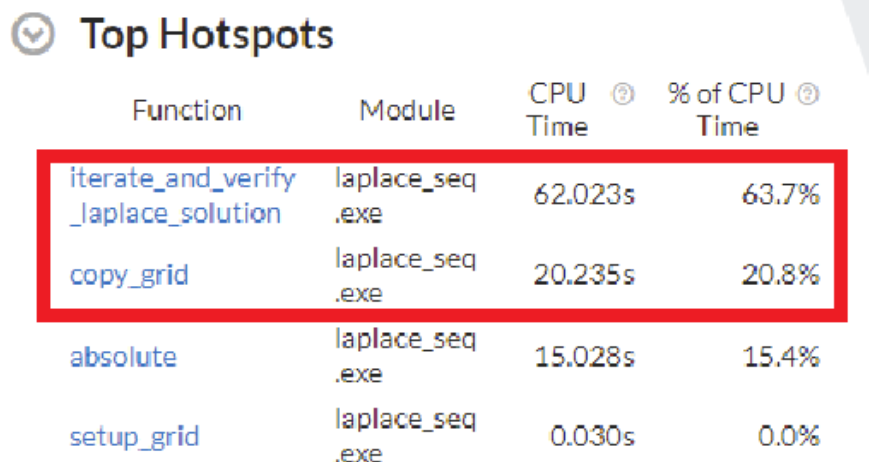
\includegraphics[width=0.48\textwidth]{images/seq_og_vtune.png}
    \caption{Análise de Desempenho da Implementação Sequencial}
    \label{fig:seq_og_vtune}
\end{figure}

Como podemos ver na Figura \ref{fig:seq_og_vtune}, a maior parte do tempo de execução é gasta na iteração de Jacobi e na cópia de matrizes. Portanto, essas duas partes do código foram as escolhidas para serem paralelizadas. Em terceiro lugar no tempo de execução está a função \texttt{absolute}, que foi substituída pela função \texttt{fabs} para melhorar o desempenho do código.

A seguir, apresentamos os resultados obtidos com a implementação sequencial e com a implementação sequencial otimizada. Durante a medição comparativa de desempenho, foram executadas 20 iterações para cada tamanho de grade.

\begin{figure}[H]
    \centering
    \begin{tikzpicture}
        \begin{axis}[
                enlargelimits=0.15,
                legend style={at={(0.5,-0.15)},
                        anchor=north,legend columns=-1},
                ylabel={Média do Tempo de Execução (s)},
                symbolic x coords={512, 1024, 2048, 4096, 8192},
                xtick=data,
                x tick label style={font=\small},
                every node near coord/.append style={font=\tiny},
            ]
            \addplot[smooth, mark=*, red] coordinates {(512,1.548) (1024,6.365) (2048,25.91) (4096,98.651) (8192,388.764)};
            \addplot[smooth, mark=*, blue] coordinates {(512,0.211) (1024,0.857) (2048,5.741) (4096,24.2) (8192,96.436)};

            \legend{Sequencial, Sequencial Otimizado}
        \end{axis}
    \end{tikzpicture}
    \caption{Comparação do tempo de execução da implementação sequencial}
    \label{fig:seq_time_line_chart}
\end{figure}

\begin{figure}[H]
    \centering
    \begin{tikzpicture}
        \begin{axis}[
                ybar,
                enlargelimits=0.15,
                legend style={at={(0.5,-0.15)},
                        anchor=north,legend columns=-1},
                ylabel={Speed Up},
                symbolic x coords={512, 1024, 2048, 4096, 8192},
                xtick=data,
                nodes near coords,
                nodes near coords align={vertical},
                x tick label style={font=\small},
                every node near coord/.append style={font=\small},
                bar width=7pt,
            ]
            \addplot coordinates {(512,7.34) (1024,7.43) (2048,4.51) (4096,4.08) (8192,4.03)};

            \legend{Sequencial Otimizado}
        \end{axis}
    \end{tikzpicture}
    \caption{Speed Up da implementação sequencial otimizada}
    \label{fig:seq_speedup_bar_chart}
\end{figure}

Como podemos ver na Figura \ref{fig:seq_time_line_chart}, a implementação sequencial otimizada é mais rápida do que a implementação sequencial original. Um dos motivos para isso é que a implementação sequencial otimizada aloca memória de forma contígua, o que garante a melhor utilização da memória cache do processador.

Outro motivo é que a implementação sequencial otimizada utiliza a função \texttt{fabs} para calcular o valor absoluto, que é otimizada para desempenho por ser implementada em linguagem de baixo nível. Além disso, a implementação sequencial otimizada utiliza a flag de compilação \texttt{-O3} para ativar um conjunto de otimizações de alto nível que podem melhorar o desempenho do código.

\subsection{Análise de Desempenho - Memória Compartilhada}

Durante a medição comparativa de desempenho, foram executadas 20 iterações para cada tamanho de grade, com a quantidade de threads fixa em 24.

\begin{figure}[H]
    \centering
    \begin{tikzpicture}
        \begin{axis}[
                enlargelimits=0.15,
                legend style={at={(0.5,-0.15)},
                        anchor=north,legend columns=-1},
                ylabel={Média do Tempo de Execução (s)},
                symbolic x coords={512, 1024, 2048, 4096, 8192},
                xtick=data,
                x tick label style={font=\small},
                every node near coord/.append style={font=\tiny},
            ]

            \addplot[smooth, mark=*, blue] coordinates {(512,0.044) (1024,0.144) (2048,2.303) (4096,12.354) (8192,43.73)};
            \addplot[smooth, mark=*, red] coordinates {(512,1.548) (1024,6.365) (2048,25.91) (4096,98.651) (8192,388.764)};

            \legend{OpenMP, Sequencial Otimizado}
        \end{axis}
    \end{tikzpicture}
    \caption{Comparação do tempo de execução da implementação sequencial e da implementação OpenMP}
    \label{fig:seq_omp_time_line_chart}
\end{figure}

\begin{figure}[H]
    \centering
    \begin{tikzpicture}
        \begin{axis}[
                ybar,
                enlargelimits=0.15,
                legend style={at={(0.5,-0.15)},
                        anchor=north,legend columns=-1},
                ylabel={Speed Up},
                symbolic x coords={512, 1024, 2048, 4096, 8192},
                xtick=data,
                nodes near coords,
                nodes near coords align={vertical},
                x tick label style={font=\small},
                every node near coord/.append style={font=\small},
                bar width=7pt,
            ]
            \addplot coordinates {(512,4.80) (1024,5.95) (2048,2.49) (4096,1.96) (8192,2.21)};

            \legend{OpenMP}
        \end{axis}
    \end{tikzpicture}
    \caption{Speed Up da implementação OpenMP com 24 threads}
    \label{fig:seq_omp_speedup_bar_chart}
\end{figure}

Como podemos ver na Figura \ref{fig:seq_omp_time_line_chart}, a implementação OpenMP é mais rápida do que a implementação sequencial otimizada. Um dos motivos para isso é que a implementação OpenMP paraleliza a iteração de Jacobi e a cópia de matrizes, que são as partes do código que mais gastam tempo de execução.

A seguir, apresentamos os resultados obtidos com a implementação OpenMP com diferentes quantidades de threads. Durante a medição comparativa de desempenho, foram executadas 20 iterações com o tamanho da grade fixo em 2048x2048.

\begin{figure}[H]
    \centering
    \begin{tikzpicture}
        \begin{axis}[
                enlargelimits=0.15,
                legend style={at={(0.5,-0.15)},
                        anchor=north,legend columns=-1},
                ylabel={Média do Tempo de Execução (s)},
                symbolic x coords={2, 4, 8, 16, 24},
                xtick=data,
                x tick label style={font=\small},
                every node near coord/.append style={font=\tiny},
            ]

            \addplot[smooth, mark=*, blue] coordinates {(2,4.064) (4,2.669) (8,2.061) (16,2.12) (24,2.303)};

            \legend{OpenMP}
        \end{axis}
    \end{tikzpicture}
    \caption{Comparação do tempo de execução da implementação OpenMP com diferentes quantidades de threads}
    \label{fig:omp_thread_line_chart}
\end{figure}

É possível observar na Figura \ref{fig:omp_thread_line_chart} que o tempo de execução diminui com o aumento da quantidade de threads, mas o desempenho não melhora significativamente com mais de 8 threads. Isso pode ocorrer pois o tamanho da grade é pequeno, então o tempo de comunicação entre as threads é maior do que o tempo de execução da iteração de Jacobi e da cópia de matrizes.

\subsection{Análise de Desempenho - Memória Distribuída com Controller/Worker}

\subsection{Análise de Desempenho - Memória Distribuída com SPMD}

\subsection{Análise de Desempenho - Cache e Gargalos}

Uma das hipóteses levantadas durante a implementação do algoritmo foi que a implementação sequencial otimizada aloca memória de forma contígua, o que garante a melhor utilização da memória cache do processador. Para confirmar essa hipótese, foi realizada uma análise de desempenho com a ferramenta \texttt{VTune} utilizando uma grade de tamanho 4096x4096.

\begin{figure}[H]
    \centering
    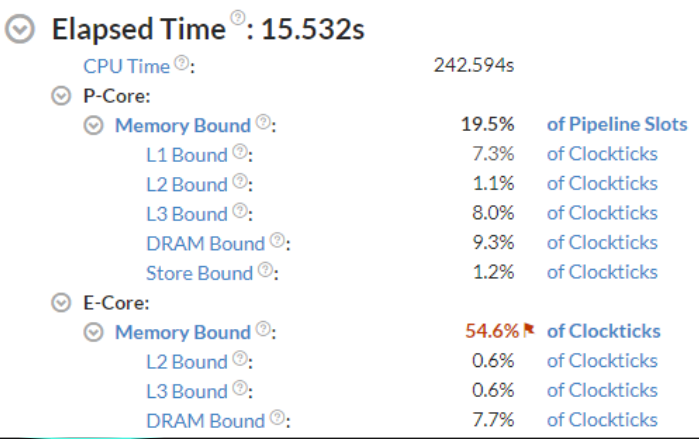
\includegraphics[width=0.48\textwidth]{images/seq_og_vtune_cache.png}
    \caption{Análise com VTune da implementação OpenMP não otimizada}
    \label{fig:seq_og_vtune_cache}
\end{figure}

\begin{figure}[H]
    \centering
    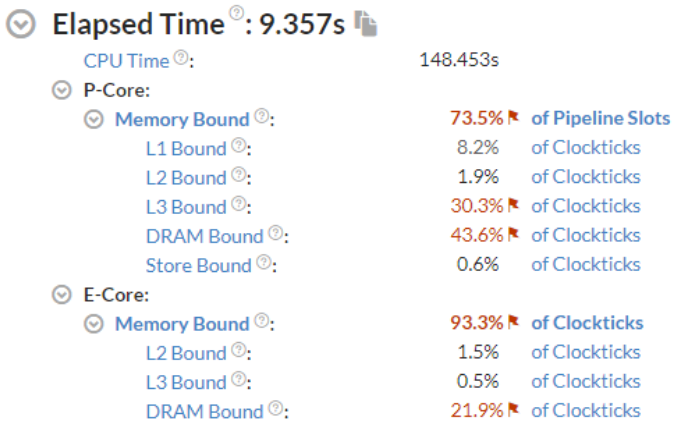
\includegraphics[width=0.48\textwidth]{images/seq_opt_vtune_cache.png}
    \caption{Análise com VTune da implementação OpenMP otimizada (localidade de memória)}
    \label{fig:seq_opt_vtune_cache}
\end{figure}

Como podemos ver nas Figuras \ref{fig:seq_og_vtune_cache} e \ref{fig:seq_opt_vtune_cache}, a implementação sequencial otimizada possui uma taxa de L1 Cache Bound maior do que a implementação sequencial original. Isso corroborar com a hipótese de que a implementação sequencial otimizada aloca memória de forma contígua, o que garante a melhor utilização da memória cache do processador. Além disso, também podemos afirmar que a performance da implementação atual está sendo limitada pela velocidade da memória RAM, ao invés ddo processador.

\section{Conclusões}

Ao longo deste trabalho, investigamos técnicas computacionais para a solução eficiente da equação de Laplace, um problema matemático com aplicações práticas em numerosos ramos tais como física, engenharia e meteorologia. Através da aplicação do método iterativo de Jacobi, chegamos a uma solução base que, apesar de sua utilidade, se mostrou limitada em termos de tempo de execução quando aplicada a grids de grandes dimensões.

Para superar tal desafio, este artigo apresentou estratégias de paralelização utilizando \texttt{OpenMP} e \texttt{MPI}. Os resultados alcançados foram incríveis: a paralelização mostrou-se capaz de diminuir de forma expressiva o tempo de processamento, otimizando a resolução mesmo em situações que exigem altos volumes de dados.

Observou-se que a implementação com memória compartilhada (\texttt{OpenMP}) proporcionou um ambiente eficaz para a paralelização em sistemas com múltiplos núcleos, enquanto o uso do MPI viabilizou a sua execução em clusters de processamento, resolvendo a desafiadora tarefa da computação distribuída.

Concluímos que a paralelização é uma arma considerável na solução de problemas de equações diferenciais parciais como a equação de Laplace em grids de grande porte. A escolha entre memória compartilhada e distribuída deve levar em consideração a infraestrutura disponível e o tamanho do problema.

Este estudo também abre caminho para pesquisas futuras no campo da otimização de algoritmos para problemas matemáticos complexos, sugerindo que o desenvolvimento contínuo dessas técnicas pode desempenhar um papel crucial na capacitação dos pesquisadores para resolver problemas cada vez mais exigentes com maior eficiência.

\section{Trabalhos Futuros}

Embora os resultados aqui apresentados demonstrem o potencial das técnicas de paralelização para a resolução da equação de Laplace, há várias direções interessantes para pesquisa futura. Primeiramente, a investigação pode ser ampliada para incluir outras técnicas e algoritmos de paralelização, como GPGPU (General-Purpose computing on Graphics Processing Units), onde a computação é realizada com o auxílio de processadores gráficos, possibilitando um aumento ainda maior na eficiência do processamento.

Outra direção promissor é a investigação e ajuste fino dos parâmetros de paralelização, como a granularidade das tarefas e a distribuição de carga entre processos ou threads, buscando um balanceamento ótimo que maximize a utilização do hardware disponível. Essa análise pode incluir a implementação de técnicas adaptativas que respondem dinamicamente às condições de execução em tempo real.

Por fim, o estudo da aplicação dessas técnicas de paralelização para resolver outras equações diferenciais parciais, com diferentes condições de contorno ou domínios mais complexos, é uma área de pesquisa extensa que pode levar a descobertas significativas para problemas computacionais desafiadores.

\bibliographystyle{IEEEtran}
\bibliography{references.bib}

\end{document}
